
\noindent\begin{minipage}{\textwidth}
    \begin{table}[H]
        \centering
        \caption{Hiperparâmetros e Resultados do Melhor Modelo - vit\_v8\_AB\_opt}
        \vspace{0.2cm}
        \resizebox{\textwidth}{!}{%
            \begin{tabular}{ll | lrrr}
                \hline
                \multicolumn{2}{c|}{\textbf{Hiperparâmetros}} & \multicolumn{4}{c}{\textbf{Métricas por Classe}} \\ \hline
                \textbf{Parâmetro} & \textbf{Valor} & \textbf{Classe} & \textbf{Precisão} & \textbf{Recall} & \textbf{F1-Score} \\ \hline
    Agendador (\$T\_0\$) & 12 & 31.2 & 0,0000 & 0,0000 & 0,0000 \\ 
Agendador de LR & CosineAnnealingWarmRestarts & 31.3 & 0,0000 & 0,0000 & 0,0000 \\ 
Architecture & vit\_b\_32 & 31.4 & 0,0000 & 0,0000 & 0,0000 \\ 
Batch Size & 32 & 32.3 & 0,0000 & 0,0000 & 0,0000 \\ 
Decaimento de Peso (WD) & 0,0125 & 32.4 & 0,0000 & 0,0000 & 0,0000 \\ 
Dropout & 0,0734 & 33.3 & 0,1667 & 0,3005 & 0,2144 \\ 
Função de Perda & CrossEntropyLoss & 41.4 & 0,0000 & 0,0000 & 0,0000 \\ 
Hidden Units & 512 & 41.5 & 0,0399 & 0,5641 & 0,0746 \\ 
Label Smoothing & 0,0358 & 42.4 & 0,0469 & 0,0441 & 0,0455 \\ 
Otimizador & AdamW & 44.4 & 0,0199 & 0,2069 & 0,0363 \\ 
\cline{3-6} 
Taxa de Aprendizado (LR) & 1,01e-05 & \textbf{Média (Macro)} & 0,0430 & 0,1068 & 0,0447 \\ 
Unfreeze Layers & 1 & \textbf{MCC} & \multicolumn{3}{c}{0,0335} \\ 
            \hline
            \end{tabular}%
        }
    \end{table}

    \begin{figure}[H]
        \centering
        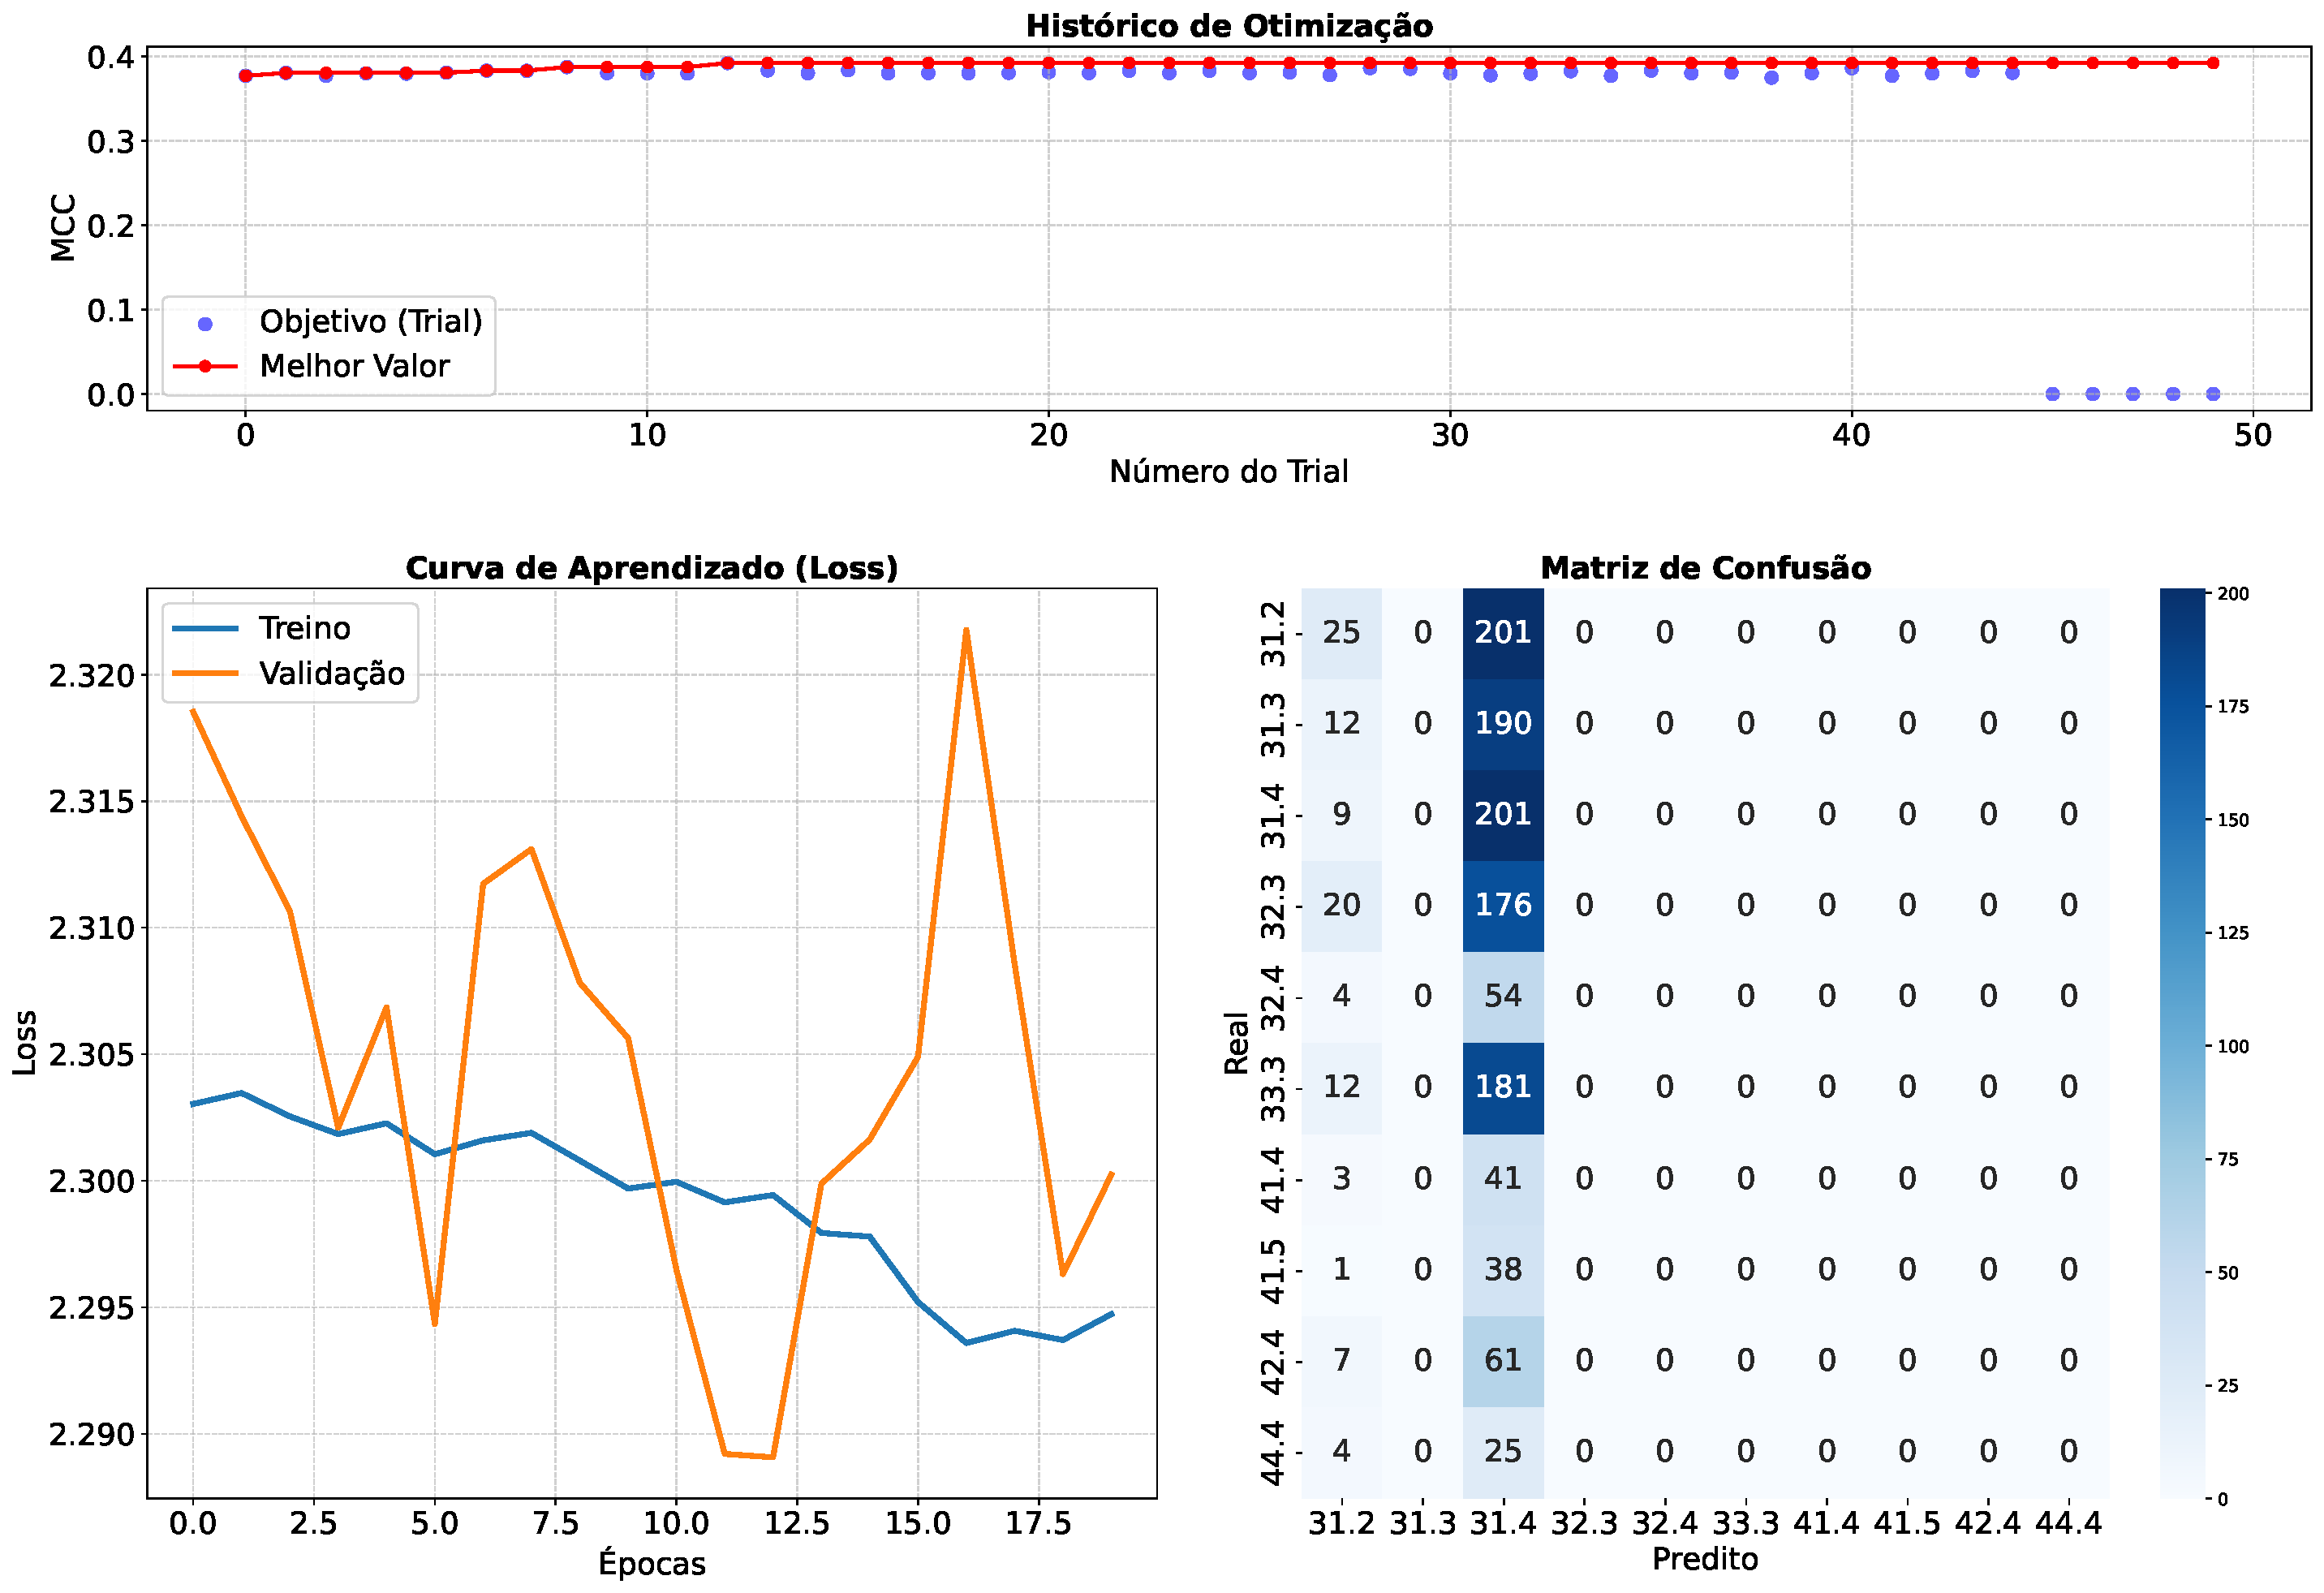
\includegraphics[width=0.85\textwidth]{tex/appendix/experiments/vit_v8_AB_opt/dashboard_consolidado.pdf}
        \caption{Histórico de Otimização, Curvas de Aprendizado e Matriz de Confusão - vit\_v8\_AB\_opt}
    \end{figure}
\end{minipage}
\clearpage
